\documentclass[conference]{IEEEtran}
\usepackage{tikz}
\usepackage{amsmath,amssymb}
\usetikzlibrary{shapes.geometric, arrows.meta, positioning, calc}

\begin{document}

\begin{figure*}[t]
\centering
\resizebox{0.97\textwidth}{!}{%
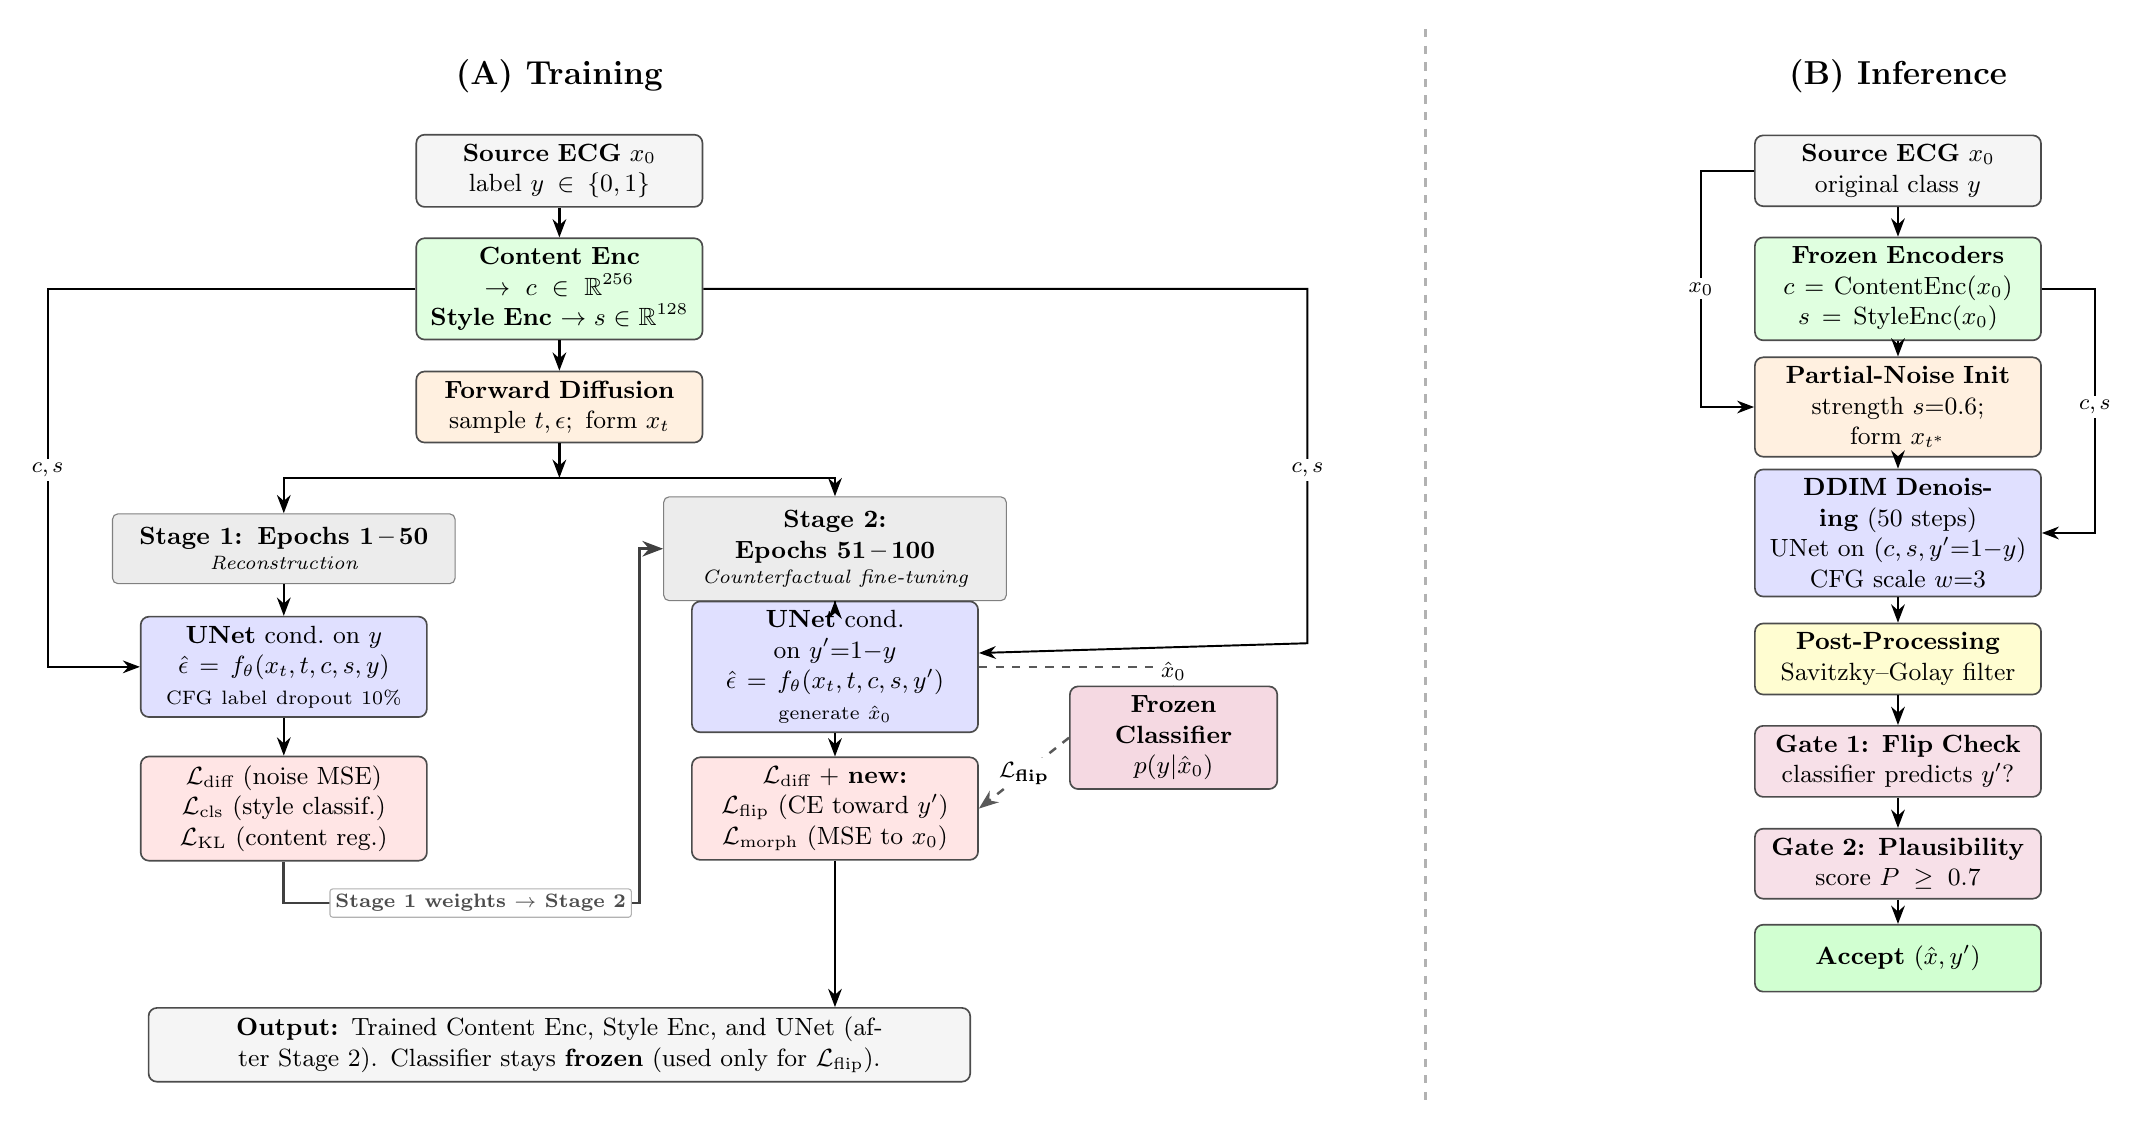
\begin{tikzpicture}[
  font=\small,
  >=Stealth,
  box/.style={rectangle, draw=black!70, rounded corners=3pt, align=center,
              minimum height=0.85cm, text width=3.4cm, fill=#1, line width=0.6pt},
  box/.default=white,
  wbox/.style={rectangle, draw=black!70, rounded corners=3pt, align=center,
              minimum height=0.85cm, fill=#1, line width=0.6pt},
  heading/.style={font=\bfseries\large},
  stagelab/.style={font=\bfseries\small, fill=gray!15, draw=black!50,
                   rounded corners=2pt, inner sep=5pt, align=center},
  arr/.style={->, line width=0.8pt, >=Stealth, color=black},
  darr/.style={->, line width=0.9pt, dashed, >=Stealth, color=black!65},
  lbl/.style={font=\footnotesize\bfseries, text=black, fill=white, inner sep=1.5pt},
]

% ============================================================
% (A) TRAINING — all absolute positions
% ============================================================
% Heading
\node[heading] at (0, 0) {(A) Training};

% Row 0: Source ECG
\node[box=gray!8] (input) at (0, -1.2) {
  \textbf{Source ECG} $x_0$\\label $y \in \{0,1\}$};

% Row 1: Encoders
\node[box=green!12] (enc) at (0, -2.7) {
  \textbf{Content Enc} $\to c \in \mathbb{R}^{256}$\\
  \textbf{Style Enc} $\to s \in \mathbb{R}^{128}$};

% Row 2: Forward Diffusion
\node[box=orange!12] (fwd) at (0, -4.2) {
  \textbf{Forward Diffusion}\\
  sample $t, \epsilon$;\, form $x_t$};

% Main vertical chain
\draw[arr] (input) -- (enc);
\draw[arr] (enc) -- (fwd);

% Branch point
\coordinate (br) at (0, -5.1);
\draw[arr] (fwd) -- (br);

% ---- STAGE 1 at x = -3.5 ----
\node[stagelab, text width=4.0cm] (s1) at (-3.5, -6.0) {
  Stage 1: Epochs 1\,--\,50\\[-2pt]
  {\normalfont\itshape\scriptsize Reconstruction}};

\node[box=blue!12] (u1) at (-3.5, -7.5) {
  \textbf{UNet} cond.\ on $y$\\
  $\hat\epsilon = f_\theta(x_t, t, c, s, y)$\\
  {\scriptsize CFG label dropout 10\%}};

\node[box=red!10] (l1) at (-3.5, -9.3) {
  $\mathcal{L}_\text{diff}$ (noise MSE)\\
  $\mathcal{L}_\text{cls}$ (style classif.)\\
  $\mathcal{L}_\text{KL}$ (content reg.)};

\draw[arr] (br) -| (s1.north);
\draw[arr] (s1) -- (u1);
\draw[arr] (u1) -- (l1);

% ---- STAGE 2 at x = +3.5 ----
\node[stagelab, text width=4.0cm] (s2) at (3.5, -6.0) {
  Stage 2: Epochs 51\,--\,100\\[-2pt]
  {\normalfont\itshape\scriptsize Counterfactual fine-tuning}};

\node[box=blue!12] (u2) at (3.5, -7.5) {
  \textbf{UNet} cond.\ on $y'{=}1{-}y$\\
  $\hat\epsilon = f_\theta(x_t, t, c, s, y')$\\
  {\scriptsize generate $\hat{x}_0$}};

\node[box=red!10] (l2) at (3.5, -9.3) {
  $\mathcal{L}_\text{diff}$ + \textbf{new:}\\
  $\mathcal{L}_\text{flip}$ (CE toward $y'$)\\
  $\mathcal{L}_\text{morph}$ (MSE to $x_0$)};

\draw[arr] (br) -| (s2.north);
\draw[arr] (s2) -- (u2);
\draw[arr] (u2) -- (l2);

% ---- FROZEN CLASSIFIER at x = +7.8, between u2 and l2 ----
\node[box=purple!15, text width=2.4cm] (clf) at (7.8, -8.4) {
  \textbf{Frozen}\\
  \textbf{Classifier}\\
  $p(y|\hat{x}_0)$};

% UNet S2 → Classifier: perfectly horizontal then vertical (L-shape)
\draw[darr]
  (u2.east) -- (clf.north |- u2.east) -- (clf.north)
  node[pos=0.25, lbl] {$\hat{x}_0$};

% Classifier → Loss S2: straight left
\draw[darr]
  (clf.west) -- (l2.east)
  node[midway, lbl] {$\mathcal{L}_\text{flip}$};

% ---- ENCODER CONDITIONING ----
% Left path: routed at x = -6.5 (well left of Stage 1)
\draw[arr, line width=0.7pt]
  (enc.west) -- (-6.5, -2.7) -- (-6.5, -7.5) -- (u1.west);
\node[lbl] at (-6.5, -5.0) {$c, s$};

% Right path: routed at x = 9.5 (well right of frozen classifier at x=7.8)
% Enters UNet slightly above center to avoid overlapping the dashed x̂₀ arrow
\draw[arr, line width=0.7pt]
  (enc.east) -- (9.5, -2.7) -- (9.5, -7.2) -- ([yshift=5pt]u2.east);
\node[lbl] at (9.5, -5.0) {$c, s$};

% ---- SEQUENTIAL ARROW: Stage 1 → Stage 2 ----
% From Stage 1 loss, down, then through the gap between stages, up into Stage 2 label
% The -| operator goes horizontal (right) first, then vertical (up) to s2.west
\draw[->, line width=1.0pt, >=Stealth, color=black!75]
  (l1.south) -- (-3.5, -10.5) -| ([xshift=-0.3cm]s2.west) -- (s2.west);
\node[font=\scriptsize\bfseries, text=black!70, fill=white, inner sep=2pt,
      draw=black!30, rounded corners=1pt]
  at (-1.0, -10.5) {Stage~1 weights $\rightarrow$ Stage~2};

% ---- OUTPUT BOX (only from Stage 2) ----
\node[wbox=gray!8, text width=10.2cm] (out) at (0, -12.3) {
  \textbf{Output:} Trained Content Enc, Style Enc, and UNet (after Stage~2).
  Classifier stays \textbf{frozen} (used only for $\mathcal{L}_\text{flip}$).};

% Arrow from Stage 2 loss (l2) straight down to output box
\draw[arr] (l2.south) -- (l2.south |- out.north);


% ============================================================
% (B) INFERENCE — all at x = 17
% ============================================================
\node[heading] at (17, 0) {(B) Inference};

\node[box=gray!8] (i0) at (17, -1.2) {
  \textbf{Source ECG} $x_0$\\original class $y$};

\node[box=green!12] (i1) at (17, -2.7) {
  \textbf{Frozen Encoders}\\
  $c = \text{ContentEnc}(x_0)$\\
  $s = \text{StyleEnc}(x_0)$};

\node[box=orange!12] (i2) at (17, -4.2) {
  \textbf{Partial-Noise Init}\\
  strength $s{=}0.6$;\, form $x_{t^*}$};

\node[box=blue!12] (i3) at (17, -5.8) {
  \textbf{DDIM Denoising} (50 steps)\\
  UNet on $(c, s, y'{=}1{-}y)$\\
  CFG scale $w{=}3$};

\node[box=yellow!18] (i4) at (17, -7.4) {
  \textbf{Post-Processing}\\
  Savitzky--Golay filter};

\node[box=purple!12] (i5) at (17, -8.7) {
  \textbf{Gate 1: Flip Check}\\
  classifier predicts $y'$?};

\node[box=purple!12] (i6) at (17, -10.0) {
  \textbf{Gate 2: Plausibility}\\
  score $P \ge 0.7$};

\node[box=green!18] (i7) at (17, -11.2) {
  \textbf{Accept} $(\hat{x}, y')$};

% Vertical chain
\draw[arr] (i0) -- (i1);
\draw[arr] (i1) -- (i2);
\draw[arr] (i2) -- (i3);
\draw[arr] (i3) -- (i4);
\draw[arr] (i4) -- (i5);
\draw[arr] (i5) -- (i6);
\draw[arr] (i6) -- (i7);

% Source → Noise Init (left arc at x = 14.5 — clear of box west edge at 15.3)
\draw[arr, line width=0.7pt]
  (i0.west) -- (14.5, -1.2) -- (14.5, -4.2) -- (i2.west);
\node[lbl] at (14.5, -2.7) {$x_0$};

% Encoders → DDIM (right arc at x = 19.5 — clear of box east edge at 18.7)
\draw[arr, line width=0.7pt]
  (i1.east) -- (19.5, -2.7) -- (19.5, -5.8) -- (i3.east);
\node[lbl] at (19.5, -4.2) {$c, s$};


% ============================================================
% SEPARATOR — vertical dashed line at x = 11
% ============================================================
\draw[dashed, line width=1.0pt, black!30]
  (11.0, 0.6) -- (11.0, -13.0);

\end{tikzpicture}
}
\caption{Overview of the proposed pipeline. \textbf{(A)~Training} proceeds in two stages: Stage~1 (epochs 1--50) trains the UNet for noise reconstruction conditioned on label $y$; Stage~2 (epochs 51--100) fine-tunes for counterfactual generation conditioned on $y'{=}1{-}y$, adding $\mathcal{L}_\text{flip}$ and $\mathcal{L}_\text{morph}$ losses. The classifier is frozen. \textbf{(B)~Inference:} partial-noise initialization, DDIM denoising with CFG, and two quality gates filter the output.}
\label{fig:architecture}
\end{figure*}

\end{document}
